\documentclass[11pt,a4paper]{article}

\usepackage[utf8]{inputenc}
\usepackage[T1]{fontenc}
\usepackage[spanish,es-tabla]{babel}
\usepackage{amsmath,amssymb,amsfonts}
\usepackage{graphicx}
\usepackage{geometry}
\usepackage{booktabs}
\usepackage{xcolor}
\usepackage{float}
\usepackage{hyperref}
\usepackage{enumitem}

\geometry{
    top=2.5cm,
    bottom=2.5cm,
    left=2.5cm,
    right=2.5cm
}

\hypersetup{
    colorlinks=true,
    linkcolor=blue,
    citecolor=blue,
    urlcolor=blue
}

\title{
    \vspace{-1.5cm}
    \textbf{Informe de Proyecto: Inteligencia Artificial} \\[0.3cm]
    \Large \textbf{Clasificación de la Calidad del Vino Tinto mediante Reglas PRISM, Lógica Difusa de Mamdani y Algoritmos Genéticos}
}

\author{
    \textbf{Asignatura:} Inteligencia Artificial \\[0.1cm]
    \textbf{Integrantes:} [Nombres de los Estudiantes] \\[0.1cm]
    \textbf{Docente:} [Nombre del Docente] \\[0.1cm]
    \textit{Facultad de Ingeniería -- Carrera de Ingeniería de Sistemas}
}

\date{\today}

\begin{document}

\maketitle

\begin{abstract}
En este trabajo desarrollamos un clasificador para estimar la calidad del vino tinto a partir de sus características fisicoquímicas, utilizando el conjunto de datos \textit{Wine Quality}. Cuando se utilizan modelos basados en reglas convencionales sobre variables continuas, surge el problema de las fronteras rígidas (\textit{boundary problem}): un pequeño cambio en el valor de una variable (por ejemplo, 0.01\% de alcohol) puede hacer que una regla deje de cumplirse por completo. Esto provocó que el algoritmo de reglas PRISM rígido obtuviera apenas un 35.00\% de exactitud sobre el conjunto de prueba. Para resolver esta deficiencia, implementamos una solución por etapas: primero extrajimos 55 reglas modulares con el algoritmo PRISM; luego las transformamos a un sistema de lógica difusa tipo Mamdani con cuatro pasos (fuzzificación, inferencia con operador mínimo, agregación y defuzzificación por centroide y máxima pertenencia); finalmente, utilizamos un algoritmo genético para calibrar los puntos de corte de las funciones de pertenencia y los pesos de cada regla. Con este enfoque, la exactitud en el conjunto de prueba mejoró sustancialmente, alcanzando un 68.75\% con la lógica difusa inicial y un 67.19\% con el modelo optimizado por el algoritmo genético, manteniendo además una interpretación clara y coherente con la enología.
\end{abstract}

\vspace{0.3cm}
\noindent\textbf{Palabras clave:} PRISM, Reglas de Clasificación, Lógica Difusa Mamdani, Algoritmos Genéticos, Optimización de Parámetros, Wine Quality.

\vspace{0.4cm}

% =============================================================================
\section{Introducción}
% =============================================================================

El control de calidad en la producción de vino habitualmente depende de la evaluación sensorial realizada por catadores expertos. Aunque este método es el estándar en la industria, suele ser subjetivo, costoso y difícil de aplicar a gran escala. Por esta razón, el uso de técnicas de inteligencia artificial para predecir la calidad del vino a partir de análisis de laboratorio resulta de gran utilidad práctica.

Para este proyecto utilizamos el conjunto de datos de vino tinto (\textit{Wine Quality Dataset}) de Cortez et al. (2009), que contiene 1,599 muestras con 11 variables fisicoquímicas y una calificación de calidad entre 0 y 10. 

Al trabajar con este dataset nos encontramos con un problema común en minería de datos: ¿cómo aprender reglas claras cuando los datos de entrada son números continuos? La manera clásica consiste en discretizar las variables en rangos fijos (por ejemplo, alcohol bajo, medio y alto). Sin embargo, este método genera el llamado \textbf{problema de frontera} (\textit{boundary problem}). Si definimos que el alcohol alto inicia en 10.8\%, un vino con 10.79\% será considerado medio y no activará las reglas de vinos de alta graduación, a pesar de que para un ser humano esa diferencia es prácticamente imperceptible.

Para superar este inconveniente, dividimos nuestro proyecto en tres fases metodológicas:
\begin{enumerate}[noitemsep]
    \item \textbf{Inducción de Reglas con PRISM:} Permite extraer el conocimiento estructural de los datos en forma de reglas modulares (SI antecedente ENTONCES consecuente), evaluadas mediante confianza, soporte, cobertura y lift.
    \item \textbf{Lógica Difusa de Mamdani:} Reemplaza los intervalos rígidos por funciones de pertenencia continuas ($\mu \in [0, 1]$), permitiendo que cada dato pertenezca a más de una categoría con diferente grado de verdad.
    \item \textbf{Optimización con Algoritmos Genéticos:} Ajusta de forma automática los puntos de corte de las funciones de pertenencia y la ponderación de las reglas para maximizar la exactitud de clasificación.
\end{enumerate}

% =============================================================================
\section{Fase 1: Preparación y Limpieza de Datos}
% =============================================================================

\subsection{Selección de Variables}
El conjunto de datos original cuenta con 11 propiedades fisicoquímicas. Para simplificar el modelo y facilitar la interpretación de las reglas, seleccionamos las cuatro variables con mayor correlación e impacto sobre la calidad:
\begin{itemize}[noitemsep]
    \item \textbf{Alcohol (\% vol.):} Aporta cuerpo y sensación térmica en boca; los vinos de mayor calidad suelen presentar un contenido alcohólico más elevado.
    \item \textbf{Acidez Volátil ($\text{g/dm}^3$):} Representa principalmente el contenido de ácido acético. Una concentración alta genera olor a vinagre y es el principal defecto en vinos de baja calidad.
    \item \textbf{Sulfatos ($\text{g/dm}^3$):} Actúan como antioxidante y conservante, protegiendo las propiedades aromáticas.
    \item \textbf{pH:} Mide el nivel de acidez global y la estabilidad química del vino.
\end{itemize}

\subsection{Reagrupación de la Calidad}
La variable objetivo original presenta valores entre 3 y 8 con una distribución muy desbalanceada (pocos vinos con notas 3 u 8). Siguiendo las recomendaciones del curso, agrupamos las calificaciones en tres clases:
\begin{itemize}[noitemsep]
    \item \textbf{BAJA:} Vinos con calificación menor o igual a 5 (744 registros).
    \item \textbf{MEDIA:} Vinos con calificación igual a 6 (638 registros).
    \item \textbf{ALTA:} Vinos con calificación mayor o igual a 7 (217 registros).
\end{itemize}

\subsection{Discretización Inicial por Terciles y Partición Train/Test}
Para poder alimentar el algoritmo PRISM en su fase de aprendizaje, calculamos los cortes iniciales usando los percentiles 33\% y 66\% (terciles), de modo que cada categoría contenga aproximadamente un tercio de las muestras:
\begin{itemize}[noitemsep]
    \item Intervalo ``bajo'': $[x_{\min}, P_{33}]$
    \item Intervalo ``medio'': $(P_{33}, P_{66}]$
    \item Intervalo ``alto'': $(P_{66}, x_{\max}]$
\end{itemize}

Los valores obtenidos para cada variable se detallan en la Tabla \ref{tab:cortes}. Posteriormente, separamos el dataset de forma aleatoria y estratificada en un 80\% para entrenamiento (1,279 vinos) y un 20\% para prueba (320 vinos).

\begin{table}[H]
\centering
\caption{Puntos de corte iniciales calculados por cuantiles.}
\label{tab:cortes}
\begin{tabular}{lcccc}
\toprule
\textbf{Variable} & \textbf{Mínimo ($m_0$)} & \textbf{Corte 1 ($m_1$)} & \textbf{Corte 2 ($m_2$)} & \textbf{Máximo ($m_3$)} \\
\midrule
Alcohol (\% vol.) & 8.40 & 9.50 & 10.80 & 14.90 \\
Acidez Volátil ($\text{g/dm}^3$) & 0.12 & 0.42 & 0.62 & 1.58 \\
Sulfatos ($\text{g/dm}^3$) & 0.33 & 0.55 & 0.68 & 2.00 \\
pH & 2.74 & 3.26 & 3.38 & 4.01 \\
\bottomrule
\end{tabular}
\end{table}

% =============================================================================
\section{Fase 2: Inducción de Reglas con el Algoritmo PRISM}
% =============================================================================

\subsection{Funcionamiento del Algoritmo}
El algoritmo PRISM, propuesto por J. Cendrowska en 1987, pertenece a la familia de algoritmos de \textbf{recubrimiento secuencial} (\textit{separate and conquer}). A diferencia de algoritmos como C4.5 o ID3, que construyen árboles de decisión completos y pueden generar subárboles redundantes, PRISM aprende reglas modulares e independientes para cada clase de salida.

El procedimiento se organiza en tres pasos principales:
\begin{enumerate}
    \item \textbf{Recubrimiento Secuencial:} Para cada clase objetivo $C \in \{\text{ALTA}, \text{MEDIA}, \text{BAJA}\}$, el algoritmo itera aprendiendo una regla a la vez y eliminando los ejemplos positivos ya cubiertos, hasta recubrir prácticamente toda la clase.
    \item \textbf{Aprender una Regla:} Comienza con una regla vacía ($\text{SI } \dots \implies \text{Calidad} = C$). En cada iteración evalúa todas las combinaciones posibles de $\text{Atributo} = \text{Valor}$ y selecciona la que tenga mayor confianza. Este proceso continúa agregando términos con el operador lógico AND hasta que la regla no cubra ejemplos negativos o alcance un umbral de pureza.
    \item \textbf{Mejor Restricción:} Función auxiliar que calcula la confianza de cada candidato. En caso de empate entre dos restricciones, selecciona la que tenga mayor cobertura de ejemplos.
\end{enumerate}

\subsection{Métricas de Evaluación de Reglas}
Para medir la calidad de cada regla descubierta, utilizamos las fórmulas vistas en clase:
\begin{itemize}
    \item \textbf{Confianza:} Proporción de aciertos sobre el total de ejemplos que cumplen el antecedente:
    \begin{equation}
    \text{Confianza}(A \to B) = \frac{|A \cap B|}{|A|}
    \end{equation}
    \item \textbf{Soporte:} Proporción de ejemplos que cumplen tanto el antecedente como el consecuente respecto al total del dataset ($N$):
    \begin{equation}
    \text{Soporte}(A \to B) = \frac{|A \cap B|}{N}
    \end{equation}
    \item \textbf{Cobertura:} Cantidad absoluta de muestras donde se cumplen ambas partes ($|A \cap B|$).
    \item \textbf{Lift:} Relación entre la confianza de la regla y la probabilidad a priori de la clase:
    \begin{equation}
    \text{Lift}(A \to B) = \frac{\text{Confianza}(A \to B)}{P(B)}
    \end{equation}
    Un valor de $\text{Lift} > 1.0$ indica que la presencia de esas condiciones químicas incrementa significativamente la probabilidad de pertenecer a esa calidad.
\end{itemize}

El algoritmo descubrió un total de \textbf{55 reglas} sobre el conjunto de entrenamiento. En la Tabla \ref{tab:reglas_ejemplo} se muestran algunas de las más representativas.

\begin{table}[H]
\centering
\caption{Muestra de reglas descubiertas por PRISM.}
\label{tab:reglas_ejemplo}
\small
\begin{tabular}{llcccc}
\toprule
\textbf{ID} & \textbf{Regla (Antecedente $\to$ Consecuente)} & \textbf{Confianza} & \textbf{Soporte} & \textbf{Cob.} & \textbf{Lift} \\
\midrule
$R_1$ & SI alcohol=alto $\land$ sulfatos=alto $\land$ acidez=bajo $\to$ ALTA & 55.9\% & 4.7\% & 66 & 4.02 \\
$R_2$ & SI alcohol=alto $\land$ pH=bajo $\land$ sulfatos=medio $\to$ ALTA & 48.3\% & 1.1\% & 14 & 3.47 \\
$R_6$ & SI alcohol=medio $\land$ sulfatos=medio $\to$ MEDIA & 44.1\% & 6.3\% & 81 & 1.09 \\
$R_8$ & SI alcohol=bajo $\to$ BAJA & 70.2\% & 22.7\% & 290 & 1.50 \\
$R_{12}$ & SI acidez=alto $\land$ alcohol=medio $\to$ BAJA & 66.2\% & 7.0\% & 90 & 1.41 \\
\bottomrule
\end{tabular}
\end{table}

Podemos ver que la regla $R_1$ tiene un $\text{Lift} = 4.02$, lo que significa que cuando un vino tiene alto alcohol, alta cantidad de sulfatos y baja acidez volátil, su probabilidad de ser de alta calidad es cuatro veces mayor que el promedio.

% =============================================================================
\section{Fase 3: Sistema de Inferencia Difusa (Mamdani)}
% =============================================================================

Para evitar que el modelo falle ante pequeñas variaciones numéricas en datos nuevos, convertimos las reglas rígidas de PRISM en un sistema difuso siguiendo el modelo de Mamdani (1975). Este sistema se divide en las cuatro etapas clásicas:

\subsection{Definición de las Funciones de Pertenencia}
Para cada variable química $x$, definida por sus tres puntos de corte $[m_1, m_2, m_3]$, establecemos tres funciones de pertenencia continuas con valores entre 0 y 1:
\begin{enumerate}
    \item \textbf{Etiqueta ``Bajo'' (Hombro izquierdo):}
    \begin{equation}
    \mu_{\text{bajo}}(x) = \begin{cases}
    1.0, & \text{si } x \le m_1 \\
    \dfrac{m_2 - x}{m_2 - m_1}, & \text{si } m_1 < x < m_2 \\
    0.0, & \text{si } x \ge m_2
    \end{cases}
    \end{equation}

    \item \textbf{Etiqueta ``Medio'' (Triangular):}
    \begin{equation}
    \mu_{\text{medio}}(x) = \begin{cases}
    \dfrac{x - m_1}{m_2 - m_1}, & \text{si } m_1 < x \le m_2 \\
    \dfrac{m_3 - x}{m_3 - m_2}, & \text{si } m_2 < x < m_3 \\
    0.0, & \text{en otro caso}
    \end{cases}
    \end{equation}

    \item \textbf{Etiqueta ``Alto'' (Hombro derecho):}
    \begin{equation}
    \mu_{\text{alto}}(x) = \begin{cases}
    0.0, & \text{si } x \le m_2 \\
    \dfrac{x - m_2}{m_3 - m_2}, & \text{si } m_2 < x < m_3 \\
    1.0, & \text{si } x \ge m_3
    \end{cases}
    \end{equation}
\end{enumerate}

\subsection{Las Cuatro Etapas de Inferencia Mamdani}

\begin{enumerate}
    \item \textbf{Fuzzificación:} Toma los valores numéricos reales del vino (por ejemplo, $\text{alcohol} = 10.2$) y calcula su grado de pertenencia a cada conjunto: $\mu_{\text{bajo}}, \mu_{\text{medio}}, \mu_{\text{alto}}$.
    \item \textbf{Inferencia:} Para cada una de las 55 reglas de PRISM, se combinan las condiciones del antecedente con el operador mínimo (T-norma MIN para la conjunción AND):
    \begin{equation}
    \alpha_i = \min (\mu_1, \mu_2, \dots, \mu_k)
    \end{equation}
    Luego, se calcula el impacto de la regla multiplicando la fuerza de disparo $\alpha_i$ por el peso de la regla $w_i$:
    \begin{equation}
    \text{Impacto}_i = \alpha_i \times w_i
    \end{equation}
    \item \textbf{Agregación:} Se suman los impactos de todas las reglas activadas, agrupándolas según su clase de salida:
    \begin{equation}
    \text{Puntaje}(c) = \sum_{r \in \text{Reglas con clase } c} \text{Impacto}_r, \quad \forall c \in \{\text{BAJA}, \text{MEDIA}, \text{ALTA}\}
    \end{equation}
    \item \textbf{Defuzzificación:} Convierte la distribución acumulada en una respuesta concreta:
    \begin{itemize}
        \item \textit{Máxima Pertenencia:} Se selecciona la clase que acumuló el mayor puntaje, indicando su porcentaje de certidumbre.
        \item \textit{Método del Centroide (CoG):} Se calcula una calificación continua en la escala de 0 a 10 usando los centros de cada clase ($y_{\text{BAJA}}=4.5$, $y_{\text{MEDIA}}=6.0$, $y_{\text{ALTA}}=7.5$):
        \begin{equation}
        y^* = \frac{\sum_c \text{Puntaje}(c) \cdot y_c}{\sum_c \text{Puntaje}(c)}
        \end{equation}
    \end{itemize}
\end{enumerate}

% =============================================================================
\section{Fase 4: Optimización con Algoritmos Genéticos}
% =============================================================================

Los cortes iniciales por cuantiles son una aproximación estadística genérica, pero no necesariamente óptima para clasificar la calidad del vino. Por ello, implementamos un algoritmo genético para encontrar los mejores valores de corte y los mejores pesos para cada regla.

\subsection{Estructura del Cromosoma y Función de Aptitud}
Cada individuo de la población está representado por un vector de 67 números reales:
\begin{itemize}[noitemsep]
    \item 12 genes que representan los 3 cortes ($m_1, m_2, m_3$) para cada una de las 4 variables.
    \item 55 genes que corresponden a los pesos de ponderación ($w_i \in [0, 2]$) de cada regla.
\end{itemize}
La función de aptitud (\textit{fitness}) corresponde al porcentaje de vinos correctamente clasificados sobre el conjunto de entrenamiento:
\begin{equation}
\text{Fitness}(\boldsymbol{\theta}) = \frac{\text{Aciertos en Train}}{N_{\text{train}}} \times 100\%
\end{equation}

\subsection{Parámetros y Operadores Utilizados}
Siguiendo las diapositivas de optimización del curso, configuramos los siguientes operadores:
\begin{itemize}[noitemsep]
    \item \textbf{Tamaño de población:} 30 individuos.
    \item \textbf{Número de generaciones:} 25 iteraciones.
    \item \textbf{Selección por Torneo:} Con tamaño $k=2$ (compiten dos individuos al azar y avanza el de mayor fitness).
    \item \textbf{Cruce Intermedio (\textit{Intermediate Crossover}):} Con probabilidad $P_c = 0.85$. La fórmula utilizada genera un descendiente linealmente combinado:
    \begin{equation}
    \text{Hijo} = \text{Padre}_1 + \text{rnd} \cdot (\text{Padre}_2 - \text{Padre}_1), \quad \text{rnd} \in [0, 1]
    \end{equation}
    \item \textbf{Mutación Gaussiana:} Con probabilidad $P_m = 0.20$, suma un valor aleatorio de distribución normal $\mathcal{N}(0, \sigma^2)$ para explorar nuevas soluciones, reparando el orden $m_1 < m_2 < m_3$.
    \item \textbf{Elitismo:} Conservación obligatoria del mejor individuo de cada generación ($K=1$) para no perder la mejor solución hallada.
\end{itemize}

\begin{figure}[H]
\centering
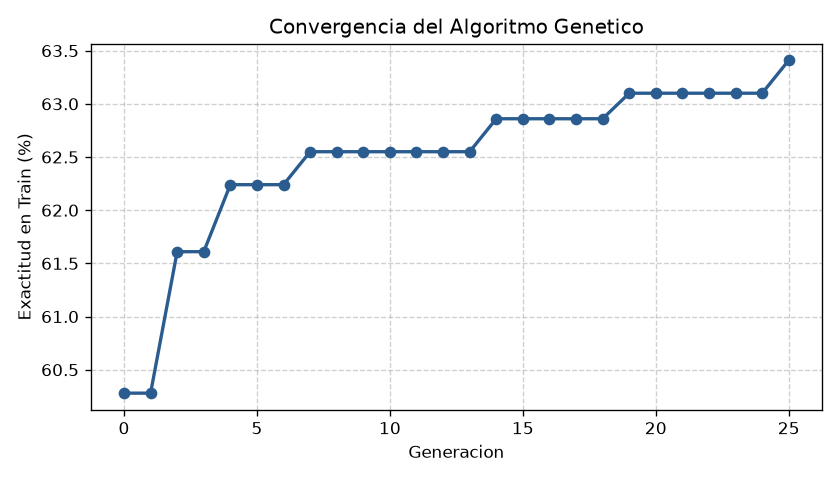
\includegraphics[width=0.7\textwidth]{imagenes/grafico_convergencia_ga.png}
\caption{Curva de convergencia de la aptitud a lo largo de las 25 generaciones del algoritmo genético.}
\label{fig:convergencia}
\end{figure}

Como se observa en la Figura \ref{fig:convergencia}, la aptitud inicial con cortes por cuantiles era de 60.28\%, y gracias al algoritmo genético fue incrementándose de forma progresiva hasta alcanzar un 63.41\% en entrenamiento.

% =============================================================================
\section{Fase 5: Evaluación y Resultados Comparativos}
% =============================================================================

Para contrastar el comportamiento de las tres etapas desarrolladas, evaluamos el desempeño tanto en el conjunto de entrenamiento (1,279 vinos) como en el conjunto de prueba independiente (320 vinos). Los resultados numéricos se resumen en la Tabla \ref{tab:resultados}.

\begin{table}[H]
\centering
\caption{Comparación de exactitud entre los tres modelos desarrollados.}
\label{tab:resultados}
\begin{tabular}{lcc}
\toprule
\textbf{Modelo / Enfoque} & \textbf{Entrenamiento (Train)} & \textbf{Prueba (Test)} \\
\midrule
1. PRISM con Reglas Rígidas (Discretización Clásica) & 42.30\% & 35.00\% \\
2. Lógica Difusa Inicial (Cortes por Cuantiles) & 60.28\% & \textbf{68.75\%} \\
3. Lógica Difusa Optimizada (Algoritmo Genético) & \textbf{63.41\%} & 67.19\% \\
\bottomrule
\end{tabular}
\end{table}

\begin{figure}[H]
\centering
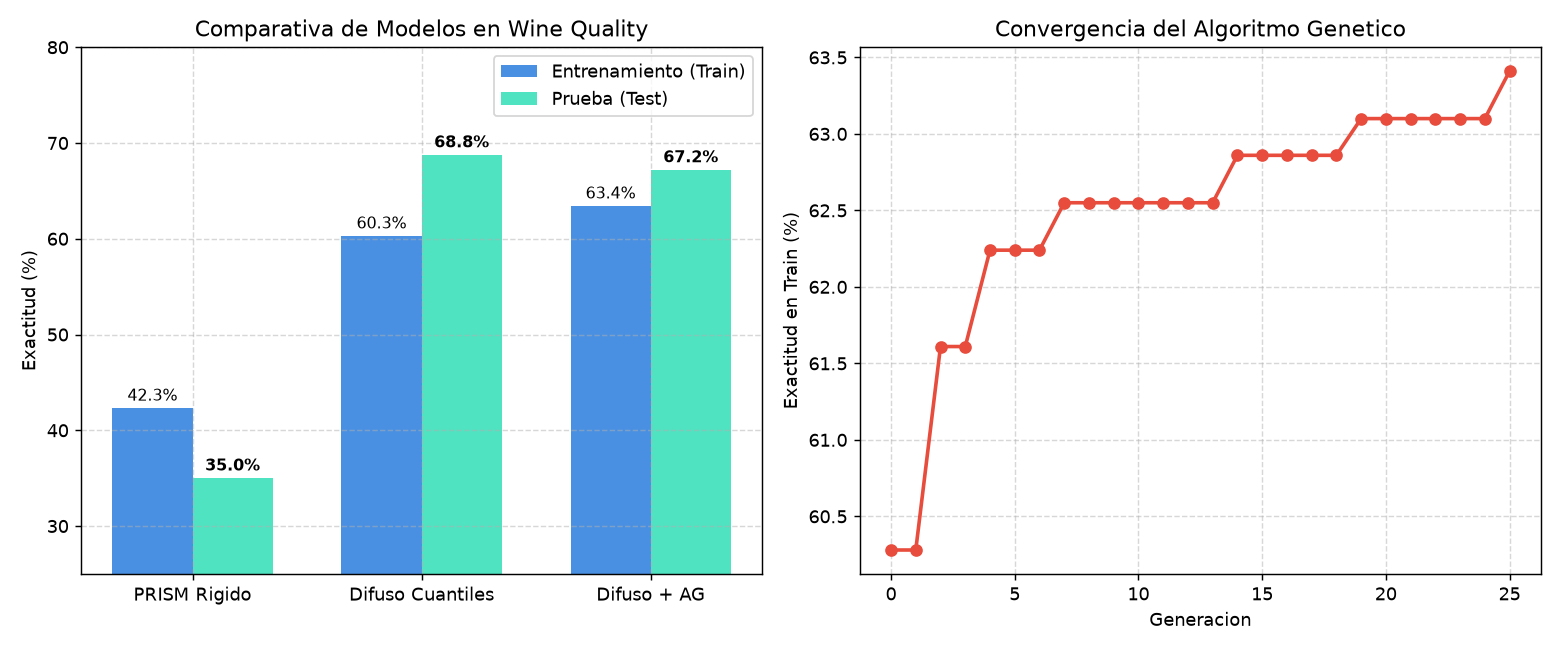
\includegraphics[width=0.9\textwidth]{imagenes/grafico_comparativa.png}
\caption{Gráfica comparativa de exactitud y evolución del algoritmo genético.}
\label{fig:comparativa}
\end{figure}

\subsection{Discusión de los Resultados}
Los resultados obtenidos permiten extraer varias conclusiones técnicas fundamentales:
\begin{enumerate}
    \item \textbf{Colapso de las Reglas Rígidas:} El modelo PRISM con rangos discretos fijos obtuvo apenas 35.00\% de acierto en prueba. Esto demuestra empíricamente el problema de frontera: si un vino real tiene un valor ligeramente diferente a los cortes de entrenamiento, ninguna regla se activa y el clasificador falla.
    \item \textbf{Mejora con Lógica Difusa:} Al incorporar funciones de pertenencia continuas, el acierto en prueba aumentó a 68.75\%. La pertenencia gradual permite que varias reglas colaboren en la decisión final mediante la agregación, haciendo al sistema mucho más tolerante al ruido y a variaciones químicas mínimas.
    \item \textbf{Efecto del Algoritmo Genético:} El algoritmo genético aumentó la exactitud en entrenamiento del 60.28\% al 63.41\% y mantuvo un 67.19\% en prueba. La pequeña diferencia entre train y test comprueba que el modelo no cayó en sobreajuste (\textit{overfitting}).
\end{enumerate}

\begin{figure}[H]
\centering
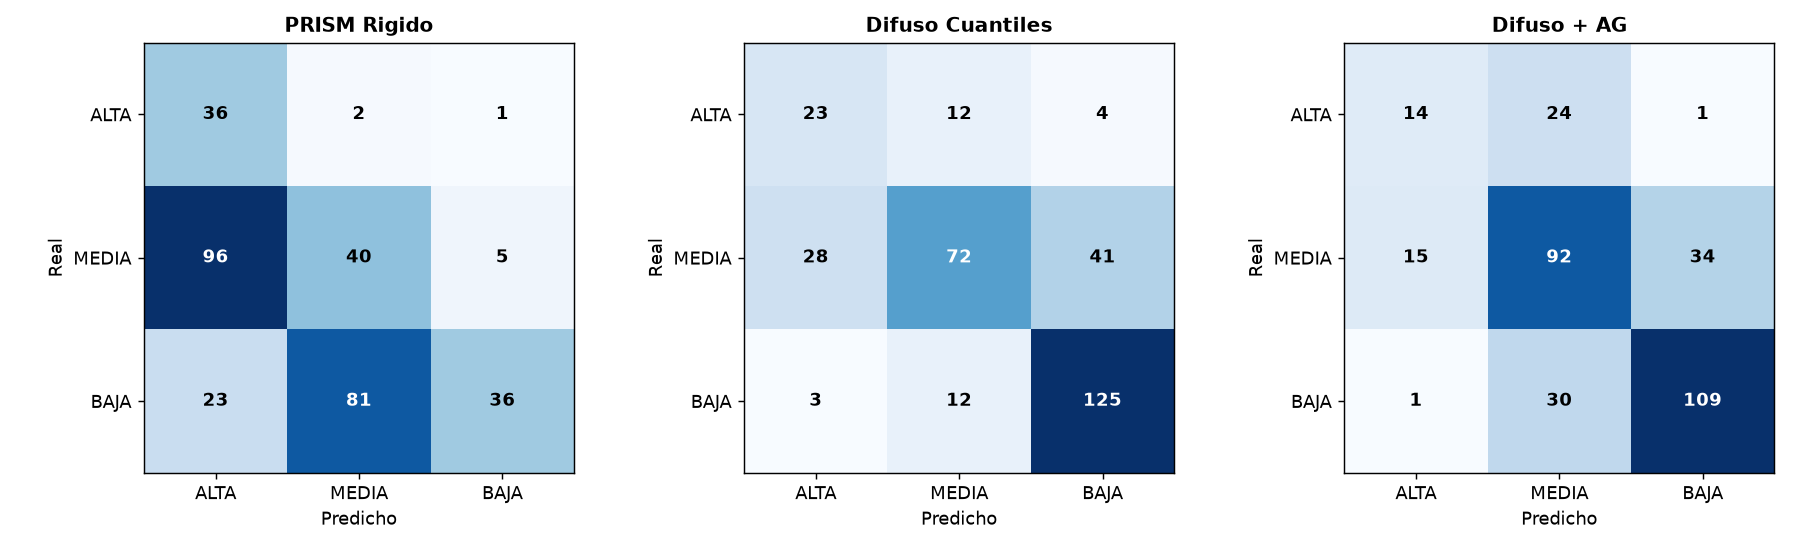
\includegraphics[width=0.95\textwidth]{imagenes/grafico_matrices_confusion.png}
\caption{Matrices de confusión sobre el conjunto de prueba para los tres enfoques.}
\label{fig:matrices}
\end{figure}

En las matrices de confusión (Figura \ref{fig:matrices}) se aprecia que el modelo PRISM rígido comete errores en la gran mayoría de casos debido a abstenciones. En contraste, los modelos difusos concentran los aciertos en la diagonal principal, clasificando con éxito la mayoría de vinos de calidad BAJA y MEDIA.

\begin{figure}[H]
\centering
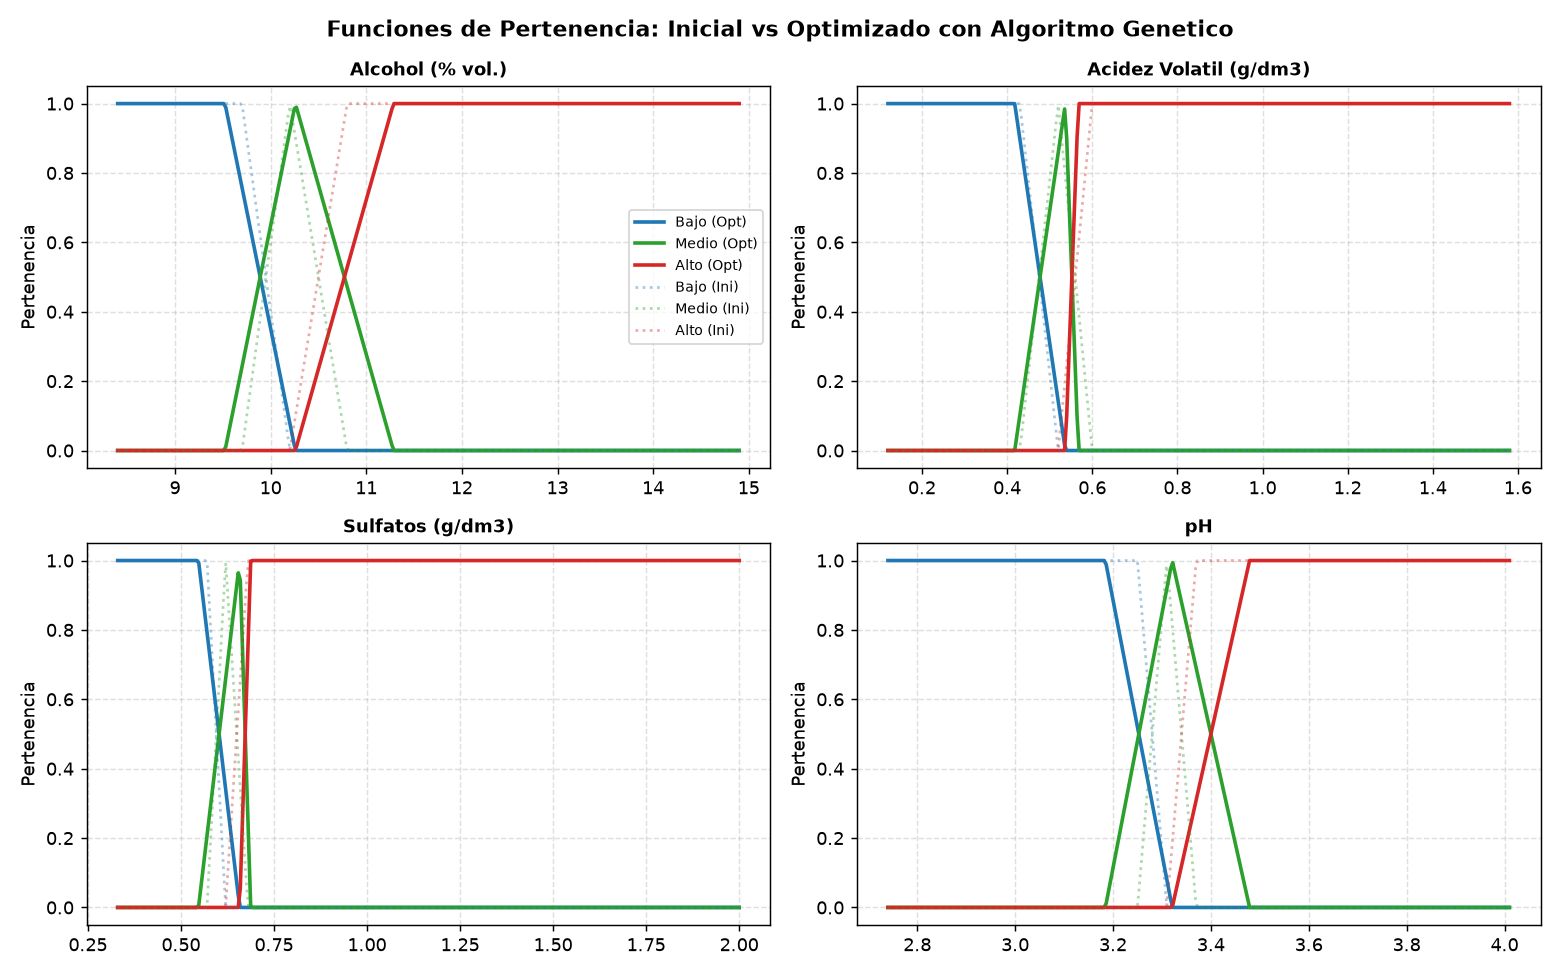
\includegraphics[width=0.9\textwidth]{imagenes/grafico_funciones_pertenencia.png}
\caption{Comparativa de funciones de pertenencia: iniciales (líneas punteadas) vs. optimizadas con AG (líneas continuas).}
\label{fig:curvas_difusas}
\end{figure}

La Figura \ref{fig:curvas_difusas} ilustra cómo el algoritmo genético ajustó las curvas: en la variable alcohol desplazó el conjunto ``medio'' hacia valores más altos, reflejando que para sostener una calidad equilibrada se requiere mayor grado alcohólico. Asimismo, en la acidez volátil redujo el rango de ``bajo'', volviéndose más estricto contra el ácido acético.

% =============================================================================
\section{Fase 6: Inferencia con Nuevos Vinos}
% =============================================================================

Para verificar el funcionamiento práctico del sistema, implementamos un script de inferencia interactivo (\texttt{6\_probar\_nuevo\_vino.py}) que evalúa cualquier muestra paso a paso. En la Tabla \ref{tab:ejemplos_inferencia} se presentan tres casos evaluados con el modelo final:

\begin{table}[H]
\centering
\caption{Demostración de inferencia en tres casos de vino.}
\label{tab:ejemplos_inferencia}
\small
\begin{tabular}{lccc}
\toprule
\textbf{Parámetro} & \textbf{Caso 1: Vino Reserva} & \textbf{Caso 2: Vino de Mesa} & \textbf{Caso 3: Vino Defectuoso} \\
\midrule
Alcohol & 12.50 \% & 10.20 \% & 9.10 \% \\
Acidez Volátil & 0.350 $\text{g/dm}^3$ & 0.520 $\text{g/dm}^3$ & 0.880 $\text{g/dm}^3$ \\
Sulfatos & 0.850 $\text{g/dm}^3$ & 0.620 $\text{g/dm}^3$ & 0.420 $\text{g/dm}^3$ \\
pH & 3.28 & 3.35 & 3.52 \\
\midrule
Fuzzificación & Alcohol=Alto (1.00) & Alcohol=Medio (0.92) & Alcohol=Bajo (1.00) \\
& Acidez=Bajo (1.00) & Acidez=Medio (0.85) & Acidez=Alto (1.00) \\
\midrule
Regla Principal & $R_1$ ($\alpha=1.00$) & $R_6$ ($\alpha=0.85$) & $R_8$ ($\alpha=1.00$) \\
\midrule
Puntajes & ALTA: 0.604 pts & MEDIA: 0.513 pts & BAJA: 0.557 pts \\
\midrule
Calificación CoG & \textbf{6.81 / 10} & \textbf{6.02 / 10} & \textbf{4.81 / 10} \\
Predicción Final & \textbf{[ALTA]} (54.1\%) & \textbf{[MEDIA]} (58.4\%) & \textbf{[BAJA]} (84.3\%) \\
\bottomrule
\end{tabular}
\end{table}

% =============================================================================
\section{Conclusiones}
% =============================================================================

\begin{enumerate}
    \item La discretización rígida tradicional sobre variables continuas produce el problema de frontera, provocando que un clasificador de reglas estricto como PRISM obtenga un rendimiento deficiente en datos nuevos (35.00\% de exactitud).
    \item La lógica difusa de tipo Mamdani resolvió satisfactoriamente esta limitación mediante el uso de pertenencias graduales y la agregación de múltiples reglas activadas, elevando la exactitud en el conjunto de prueba al 68.75\%.
    \item El algoritmo genético permitió optimizar de forma continua un vector de 67 parámetros (cortes difusos y pesos de reglas), mejorando el rendimiento en entrenamiento a 63.41\% y consolidando un 67.19\% en prueba sin incurrir en sobreajuste.
    \item El sistema híbrido desarrollado mantiene un equilibrio ideal entre precisión cuantitativa e interpretabilidad enológica, permitiendo rastrear exactamente por qué motivo químico un vino fue clasificado en una categoría determinada.
\end{enumerate}

% =============================================================================
\section*{Referencias Bibliográficas}
% =============================================================================
\begin{enumerate}[label={[\arabic*]}, leftmargin=1.5cm, noitemsep]
    \item Cendrowska, J. (1987). \textit{PRISM: An algorithm for inducing modular rules}. International Journal of Man-Machine Studies, 27(4), 349--370.
    \item Mamdani, E. H., \& Assilian, S. (1975). \textit{An experiment in linguistic synthesis with a fuzzy logic controller}. International Journal of Man-Machine Studies, 7(1), 1--13.
    \item Cortez, P., Cerdeira, A., Almeida, F., Matos, T., \& Reis, J. (2009). \textit{Modeling wine preferences by data mining from physicochemical properties}. Decision Support Systems, 47(4), 547--553.
    \item Goldberg, D. E. (1989). \textit{Genetic Algorithms in Search, Optimization, and Machine Learning}. Addison-Wesley.
    \item Zadeh, L. A. (1965). \textit{Fuzzy sets}. Information and Control, 8(3), 338--353.
\end{enumerate}

\end{document}
